\let\negmedspace\undefined
\let\negthickspace\undefined

\documentclass[journal]{IEEEtran}
\usepackage[a5paper, margin=10mm, onecolumn]{geometry}
\usepackage{tfrupee}

\setlength{\headheight}{1cm}
\setlength{\headsep}{0mm}

\usepackage{gvv-book}
\usepackage{gvv}
\usepackage{cite}
\usepackage{amsmath,amssymb,amsfonts,amsthm}
\usepackage{algorithmic}
\usepackage{graphicx}
\usepackage{textcomp}
\usepackage{xcolor}
\usepackage{txfonts}
\usepackage{listings}
\usepackage{enumitem}
\usepackage{mathtools}
\usepackage{gensymb}
\usepackage{comment}
\usepackage[breaklinks=true]{hyperref}
\usepackage{tkz-euclide} 
\usepackage{listings}
\def\inputGnumericTable{}                                 
\usepackage[latin1]{inputenc}                                
\usepackage{color}                                            
\usepackage{array}                                            
\usepackage{longtable}                                       
\usepackage{calc}                                             
\usepackage{multirow}                                         
\usepackage{hhline}                                           
\usepackage{ifthen}                                           
\usepackage{lscape}
\begin{document}

\bibliographystyle{IEEEtran}
\vspace{3cm}

\title{8.4.13}
\author{EE25BTECH11010 - Arsh Dhoke}
{\let\newpage\relax\maketitle}

\renewcommand{\thefigure}{\theenumi}
\renewcommand{\thetable}{\theenumi}
\setlength{\intextsep}{10pt}
\numberwithin{equation}{enumi}
\numberwithin{figure}{enumi}
\renewcommand{\thetable}{\theenumi}

\parindent 0px
\textbf{Question}:\\
Let a hyperbola passes through the focus of the ellipse 
$
\frac{x^2}{25} + \frac{y^2}{16} = 1.
$
The transverse and conjugate axes of this hyperbola coincide with the major and minor axes of the given ellipse, also the product of eccentricities of given ellipse and hyperbola is 1, then
\begin{multicols}{2}
\begin{enumerate}
    \item the equation of hyperbola is 
    $\frac{x^2}{9} - \frac{y^2}{16} = 1$
    \item the equation of hyperbola is 
    $\frac{x^2}{9} - \frac{y^2}{25} = 1$
    \item focus of hyperbola is $(5, 0)$
    \item vertex of hyperbola is $(5\sqrt{3}, 0)$
\end{enumerate}
\end{multicols}

\solution \\

The general equation of the conic can be written as:
\begin{align}
\vec{x^T}\vec{V}\vec{x} + 2\vec{u^T}\vec{x} + f = 0
\end{align}

\begin{align}
\vec{V}_E=\myvec{\frac{1}{25}&0\\0&\frac{1}{16}}, \quad \vec{u}=\vec{0}, \quad f=-1
\end{align}

\begin{align}
\lambda_1=\frac{1}{25}, \quad \lambda_2=\frac{1}{16}
\end{align}

\begin{align}
e_E^2 = 1 - \frac{\lambda_1}{\lambda_2}  \\
e_E = \frac{3}{5}
\end{align}

\begin{align}
e_H \cdot e_E = 1 \Rightarrow e_H = \frac{5}{3}, \quad e_H^2 = \frac{25}{9}
\end{align}

\begin{align}
\vec{V}_H = \myvec{\lambda_1' & 0 \\ 0 & \lambda_2'}, \quad f = -1
\end{align}

Hyperbola passes through  (3,0),thus
\begin{align}
9\lambda_1' - 1 = 0 \Rightarrow \lambda_1' = \frac{1}{9}
\end{align}

\begin{align}
e_H^2 = 1 - \frac{\lambda_1'}{\lambda_2'} \Rightarrow \lambda_2' = \frac{\lambda_1'}{1 - e_H^2}
\end{align}

\begin{align}
\lambda_2' = \frac{\frac{1}{9}}{1 - \frac{25}{9}} = \frac{\frac{1}{9}}{-\frac{16}{9}} = -\frac{1}{16}
\end{align}

\begin{align}
\vec{V}_H = \myvec{\frac{1}{9} & 0 \\ 0 & -\frac{1}{16}}
\end{align}

\begin{align}
\frac{x^2}{9} - \frac{y^2}{16} = 1
\end{align}

\begin{align}
b'^2 = 16, \\
c = \sqrt{\frac{\abs{\lambda_1' - \lambda_2'}}{\abs{\det{\vec{V}}}}}
\end{align}
\begin{align}
    c=5
\end{align}

\begin{align}
\text{Foci: } \myvec{\pm5 \\ 0}, \quad \text{Vertices: } \myvec{\pm3 \\ 0}
\end{align}

\begin{align}
\boxed{\text{Correct options: (1) and (3)}}
\end{align}

\begin{figure}[ht!]
\centering
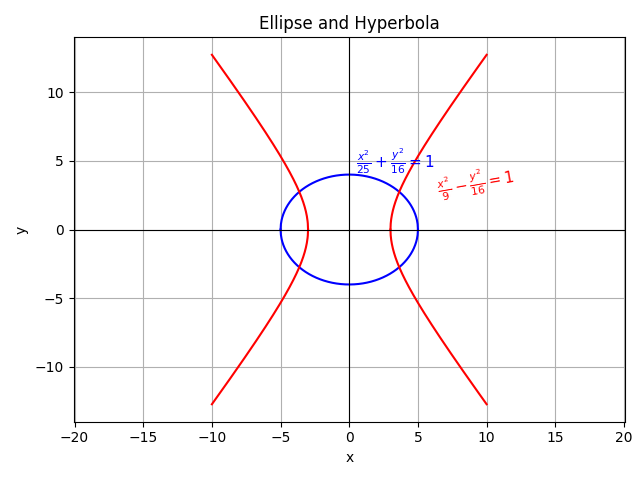
\includegraphics[height=0.4\textheight, keepaspectratio]{figs/ell.png}
\captionof{figure}{Graph}
\end{figure}

\end{document}